%
%  Simulations
% =============
%

\chapter{Simulation Method}
\label{Ch:SimS}

The work presented in this thesis has been performed using simulations with two particle-in-cell (PIC) codes:
OSIRIS~\cite{fonseca:2002} and QuickPIC~\cite{an:2013, huang:2006}.
OSIRIS is a proprietary full PIC code available in 1, 2 and 3 dimensions, with a choice between Cartesian and cylindrical coordinates.
QuickPIC is a quasi-static 3D PIC code, that is available in an open source version~\cite{add:quickpic:web}.
In the simulations presented here, both OSIRIS and the open source version of QuickPIC has been used.
For a more detailed description of PIC codes, see Appendix~\ref{Apx:PIC}.

Although PIC codes use macro particles -- that is, simulated particles representing more than one physical bunch or plasma particle -- these codes require a lot of CPU power.
This is especially true when running 3D simulations.
The preliminary studies presented in Publications~\ref{Pub:IPAC15} and~\ref{Pub:NAPAC16} were done using OSIRIS with 2D cylindrical coordinates.
The main study, Publication~\ref{Pub:BL17}, was done using QuickPIC in 3D Cartesian coordinates.
In order to perform the detailed parameter scans needed for these studies, the drive bunch and accelerating structure had to be scaled down into a more manageable size than simulating the full SPS proton bunch would require.
The full SPS proton bunch is orders of magnitude longer than both the electron bunch and the plasma wavelength, as can be seen in Table~\ref{T:AWAKERuns}.
This chapter will outline the simulation environment chosen for these studies, and the reasons behind these.

% ================================================================================================================================ %
\section{Simulating the Drive Bunch}
\label{Sim:PBeam}

An initial set of simulations were run to study the evolution of the self-modulation instability in the SPS proton bunch.
These simulations assumed the plasma was ionised at the centre of the bunch (see Section~\ref{Int:DBeam:SMI}), so only the back half of it was actually simulated.
The bunch profile function used took the form:
\begin{equation}
    f(\xi,r) = \frac{A_{q}}{2} \left[1 + \cos\left(\xi\frac{\pi}{L}\right)\right] \exp\left(-\frac{r^{2}}{2\sigma_{r}^{2}}\right), \label{EQ:SPS-Profile}
\end{equation}
where $L = 2.5\,\sigma_{z,pb} = 30\unit{cm}$ is the length of half an SPS proton bunch, $r$ and $\xi$ are the cylindrical coordinates of the simulation box (see Equation~\ref{EQ:Xi}), and $A_{q}$ is a charge scaling factor such that the total charge of the half bunch matches the charge outlined in Table~\ref{T:AWAKERuns}.
The charge of the simulated proton bunch in cylindrical coordinates is given by:
\begin{equation}
    Q_{pb} = 2\pi \iint f(\xi,r) \;r \deriv r \deriv \xi. \label{EQ:SPS-Charge}
\end{equation}
A half period cosine function for the longitudinal density profile is more convenient for simulations than a Gaussian shape, as the cosine goes to zero at a finite length~\cite{lotov:2010}.
Radially, the bunch is still Gaussian, and requires a manual cut-off to be applied to prevent OSIRIS from generating macro particles with small weights.
The CPU cost is proportional to the number of simulation particles, regardless of weight.
An example of the SPS proton bunch before and after self-modulated has occurred, as simulated in OSIRIS 3.0, can be seen in Figure~\ref{Fig:Sim:SMI}.

\begin{figure}[hbt]
    \centering
    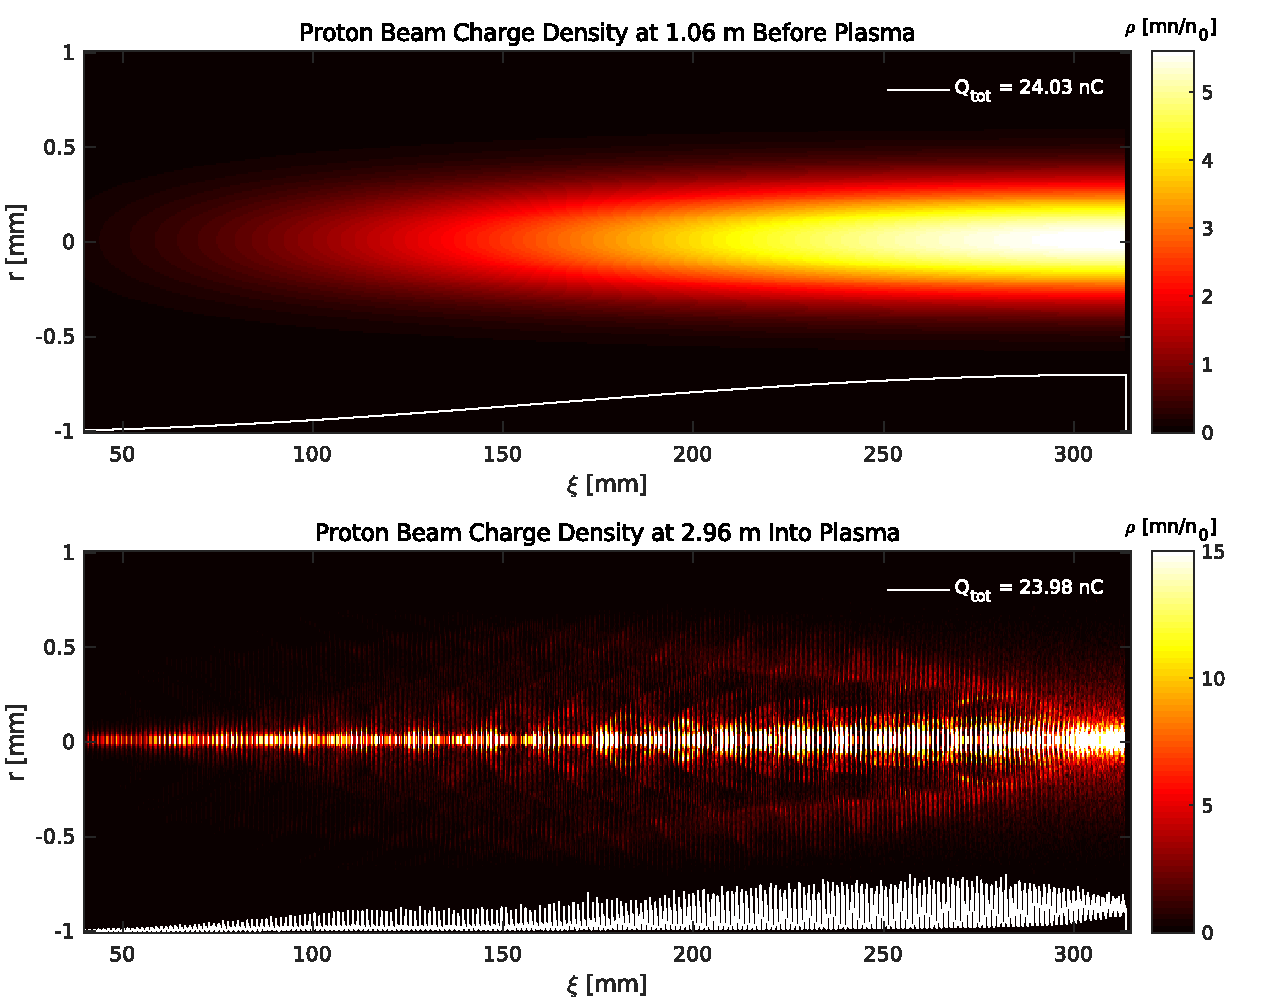
\includegraphics[width=1.0\linewidth]{figures/PBSelfModulationBefAft}
    \caption{\label{Fig:Sim:SMI}
        \textbf{Top:} An example of a simulation of half SPS proton bunch before reaching plasma.
        \textbf{Bottom:} The same bunch after having undergone self-modulation in about $3\unit{m}$ of plasma.
        The halo of protons ejected from the defocusing regions can be clearly seen, leaving a core of micro bunches on the beam axis.
        The projected density profile is shown in white.
    }
\end{figure}

% ================================================================================================================================ %

\subsection{With a Pre-Modulated Beam}
\label{Sim:PBPreMod}

The half SPS proton bunch is about $30\unit{cm}$ long, or $238\,\lambda_{pe}$, which requires a large number of grid cells to resolve, $\Delta z \gtrsim \lambda_{pe}/10$.
In order to make the simulations more manageable in size for the beam loading studies, we decided to study a sample proton bunch of 26 micro bunches -- an order of magnitude smaller than the previous case.

These simulations were all done using OSIRIS~3.0.
With this version it is necessary for the bunches to drift in vacuum for a short distance for the electro-magnetic fields to develop properly, as they are initialised at zero (see further discussion in Section~\ref{PIC:Full}).
Since the evolution of the self-modulation instability was not of primary interest at this stage, we chose to modify the bunch profile to emulate a section of the modulated bunch.
We refer to this as \textit{pre-modulation}.
This was done by shortening the period of the density envelope cosine function from Equation~\ref{EQ:SPS-Profile} to match that of the plasma wavelength,
\begin{equation}
    f(\xi,r) = A\sqrt{2} \left[\frac{1}{2\sqrt{2}}
             + \cos\left(k_{pe}\xi - \mu\right)\right] \exp\left(-\frac{r^{2}}{2\sigma_{r}^{2}}\right), \label{EQ:PB-PreMod}
\end{equation}
where $\mu$ is the position of the first micro bunch, and $k_{pe}$ is the plasma wave number~\cite{berglyd_olsen:2015}.
The offset of the cosine function is chosen such that the width of the micro bunch matches the width of a bunch in the simulations done with a full SPS bunch, and there is a gap between the bunches that approximates the gaps we see between micro bunches in the simulated self-modulated case.
Since OSIRIS ignores profile densities with negative values, the profile is automatically clipped at $0$, requiring no further manipulation of the profile function to remove negative values.

Again, cosines are preferred over a series of Gaussian bunch profiles, although this time because the cosine is periodic, and because OSIRIS' mathematical functions cannot be longer than 256 characters.

Generating an equidistant bunch train in this manner causes the head of the second bunch to be partially defocused, causing a decay of the micro bunches by the wakefield of the first bunch.
This effect was not directly compensated for in Publication~\ref{Pub:IPAC15}.
This can be avoided by increasing the separation between the first and second bunch from $2\pi c/\omega_p$ to $(2\pi+\pi/4) c/\omega_p$~\cite{lotov:2018}.

The charge of the proton micro bunches was matched to that of a micro bunch generated by the self-modulation instability in the initial simulations.
The charge density decreases towards the back end of the self-modulated bunch (see Figure~\ref{Fig:Sim:SMI}), so for the pre-modulated set-up the densities of the micro bunches were fixed to a charge for the region were the injection of an electron bunch is reasonable -- that is, around 100 plasma wavelengths behind the laser pulse.
For the pre-modulated simulations, this charge was set to $100\unit{pC}$ such that the total charge of the sample proton beam was $2.6\unit{nC}$.
This corresponds to a peak current of $135\unit{A}$.
The electron witness bunch was injected between bunch 20 and 21.

\begin{figure}[hbt]
    \centering
    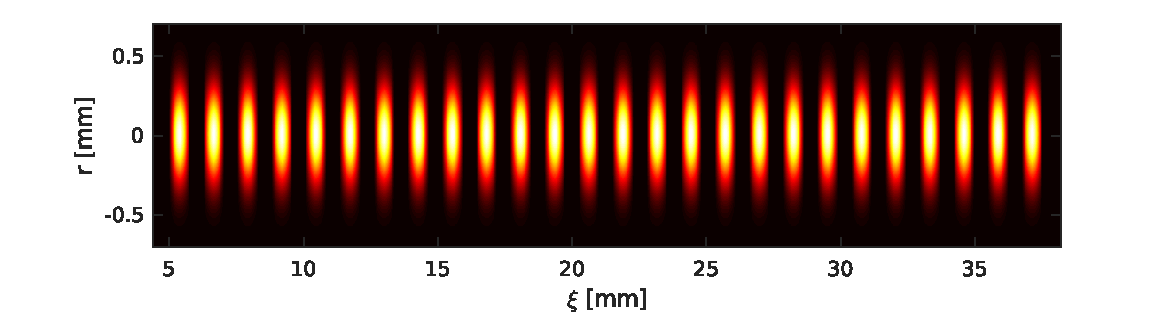
\includegraphics[width=0.9375\linewidth,trim={0mm 0mm 0mm 0mm},clip]{figures/PBPreMod}
    \caption{\label{Fig:PBPreMod}
        An example of a pre-modulated beam of 26 micro-bunches modulated at the plasma wavelength.
        This simulation set-up was used for Publication~\ref{Pub:IPAC15}.
        The density function (see Equation~\ref{EQ:PB-PreMod}) is tuned to match the earlier self-modulation simulations shown in Figure~\ref{Fig:Sim:SMI}.
    }
\end{figure}

% ================================================================================================================================ %

\subsection{With a Single Drive Bunch}
\label{Sim:PBSingle}

Further approximations needed to be made to decrease the scale of the problem in order to study the beam loading and evolution of the electron witness bunch more directly.
Even the pre-modulated proton beam is somewhat costly to simulate -- both because it still requires a multiple plasma-wavelength simulation box length, and because a large number of simulated particles are needed to populate the beam profile.
It proved to be challenging to do larger parameter scans as the CPU cost would rise to levels beyond available resources.
While additional resources could potentially have been requested, we chose instead to exclude the evolution of the proton bunch entirely from our studies and assume the region where the electron bunch was injected to have the properties laid out in the AWAKE status reports~\cite{awake_collaboration:2016}.

In these single bunch studies we therefore approximated the proton drive beam ahead of the witness bunch injection region as a single, ideal proton drive bunch generating the expected wakefields.
To reproduce these conditions, we used a Gaussian bunch of $1.46\nexp{10}$ protons corresponding to $2.34\unit{nC}$, a length $\sigma_{z} = 40\unit{\mu m}$ corresponding to $7\unit{kA}$, and a transverse size $\sigma_{x,y}=200\unit{\mu m}$~\cite{berglyd_olsen:2018}.
To prevent the proton bunch from evolving at the time scale we were interested in for these studies -- up to $100\unit{m}$ of plasma -- we also increased the mass of the bunch protons by a factor of $1\nexp{6}$.
This effectively froze the wakefields both longitudinally and transversely, and the only evolution of the wakefields was that which was caused by the electron witness bunch itself.

\begin{figure}[hbt]
    \centering
    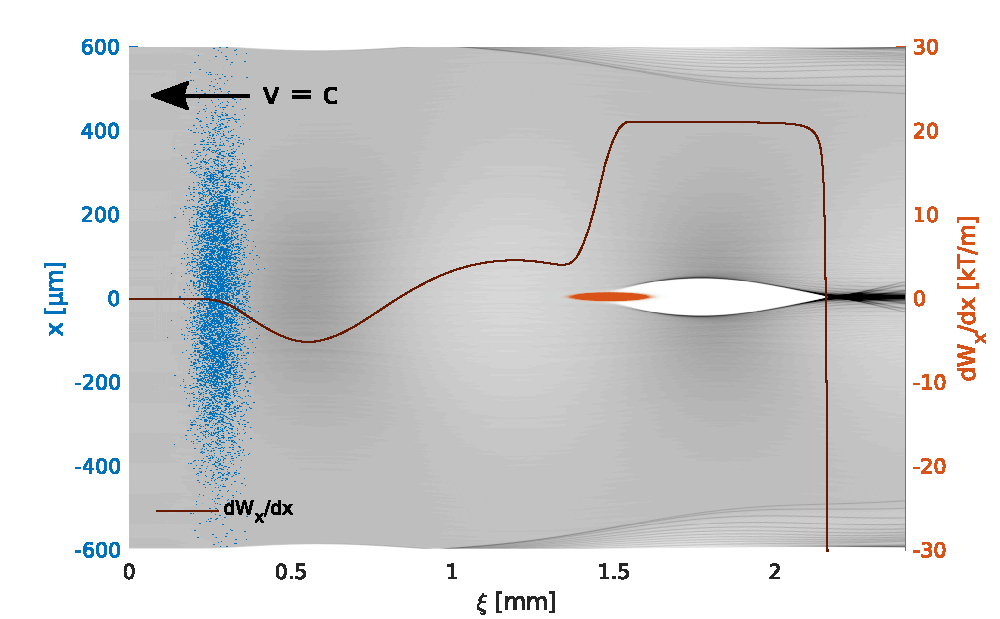
\includegraphics[width=0.8125\linewidth,trim={0mm 0mm 0mm 0mm},clip]{figures/SingleBunchPB}
    \caption{\label{Fig:PBSingle}
        An example of the simulation set-up used for Publication~\ref{Pub:BL17}.
        These simulations used a single, rigid proton bunch in blue, with a charge large enough to generate a wakefield equivalent to what we expect from the SPS proton bunch in AWAKE Run~2.
        The electron witness bunch is shown in red, and the plasma density is shown in grey where the white region is the plasma bubble void of plasma electrons.
        Note that in the QuickPIC simulations the simulation box travels towards the left.
    }
\end{figure}

Figure~\ref{Fig:PBSingle} shows the simulation setup that was used for Publication~\ref{Pub:BL17}, and shows both the proton bunch in blue, and the electron bunch in red.
The plasma can be seen as a grey shaded area where the regions void of plasma electrons can be seen in white.
This is mainly the bubble driven by the high charge density electron bunch, but also as ripples on the edge of the plasma channel.
The density perturbation and longitudinal wakefield generated by the proton bunch falls in the quasi-linear regime, as illustrated in Figures~\ref{Fig:BPI:Regime} and~\ref{Fig:BPI:Density}.

% ================================================================================================================================ %
\section{Simulating the Witness Bunch}
\label{Sim:EBeam}

Simulating the witness bunch is generally straightforward, as we have only considered a single bunch with a Gaussian shape both longitudinally and transversely.
However, there are a few things to keep in mind when setting up the bunch profile.

% ================================================================================================================================ %
\subsection{Witness Bunch Size and Resolution}
\label{Sim:EBeam:SizeRes}

For the early simulations, a transverse size of $\sigma_{x,y}=105\unit{\mu m}$ was used, see Table~\ref{T:AWAKERuns}.
For later simulations, when the bunch transverse size was matched to its emittance and the plasma density (see Section~\ref{Int:BPI:Match}), much narrower bunches were used -- on the order of a few micrometres.
The proton drive bunch size is tied to the plasma skin depth (see Section~\ref{Int:DBeam:SMI}), which is $200\unit{\mu m}$.
This, naturally, poses a resolution challenge when very narrow electron bunches need to be resolved, while at the same time, the simulation box needs to also be able to contain the proton drive bunch.
PIC codes with non-equidistant meshing are currently being developed to handle this challenge, but this option wasn't available in the simulation tools we had available.

For the simulations with a pre-modulated proton beam, used for Publication~\ref{Pub:IPAC15}, the simulation box had a radius of $2.12\unit{mm}$ with $425$ grid cells, resulting in a resolution of $5\unit{\mu m}$.
This is more than sufficient to resolve and contain both the proton beam and the electron bunch, with a small buffer for the plasma (see Section~\ref{Sim:Plasma}).
For the single drive bunch studies, Publications~\ref{Pub:NAPAC16} and~\ref{Pub:BL17}, the transverse grid resolution had to be increased.
In most cases we tried to resolve the witness bunch with at least $5$ grid cells per $\sigma_{x,y}$, although this was in some instances increased.
It was also important to keep an eye on the distribution of macro particles on the simulation grid.
This was especially important for the OSIRIS 3.0 based simulations, as OSIRIS creates macro particles of varying charge, with a fixed number of particles per cell defined by input parameters.
Since most OSIRIS simulations were run with a 2D cylindrical geometry, a $1/r$ factor enters into the electromagnetic field equations.
This results in numerical noise when $r \to 0$, which in return affects the evolution of the bunch itself.
A sample of the 2D cylindrical simulations were re-run with 3D Cartesian coordinates in order to check that the results were not dominated by this noise.
While the 3D simulations were much smoother along the beam axis, the actual results did not seem to differ to any significant degree.

QuickPIC uses 3D Cartesian coordinates, and thus, as OSIRIS 3D, does not have the $1/r$ problem.
In addition, QuickPIC has a fixed charge per macro particle, and instead varies the number of these per grid cell to create a charge distribution.
A convergence scan of resolution dependency was performed for Publication~\ref{Pub:BL17} to check that the results did not depend on resolution within the range we used for this study. The convergence scan is described in Section~\ref{SimA:Converge}.
QuickPIC defines resolution in exponents of $2$, and thus are locked to a set of values that rapidly increase for each step.
The simulations used for Publication~\ref{Pub:BL17} were done with transverse grids of $2^{9}$ and $2^{10}$ ($512 \times 512$ and $1024 \times 1024$) cells, resolving a box size of $1.2\unit{mm}$ square.
In the former case, the grid cell size was thus as large as $2\unit{\mu m}$ for the former case, and $1\unit{\mu m}$ for the latter.
This did, however, not appear to have any significant impact on the results.

Further details on how QuickPIC and OSIRIS handle bunch particles is covered in Appendix~\ref{Apx:PIC}.

% ================================================================================================================================ %
\subsection{Witness Bunch Transverse Evolution}
\label{Sim:EBeam:TEvol}

In OSIRIS~3.0, the electromagnetic fields are initialised at zero.
It is therefore necessary to let the bunches drift a short distance before they enter the plasma region for the fields to develop.
Due to this initial drift stage, it was technically challenging to inject an electron witness bunch while strictly controlling parameters like emittance, energy spread and transverse size as these parameters undergo evolution during this initial drift.
It is, however, possible to prevent the bunch from evolving by slowly ramping up the charge or the energy.
During these ramping stages the macro particles are prevented from transverse evolution.

For the early studies, and for Publication~\ref{Pub:IPAC15}, only beam loading and acceleration were considered.
For Publications~\ref{Pub:NAPAC16} and~\ref{Pub:BL17} it was, however, necessary to control the witness bunch emittance.
While QuickPIC has input parameters defining the bunch emittance in each direction, OSIRIS~3.0 does not.
OSIRIS~3.0 does let one define spatial and momentum distributions independently (see Appendix~\ref{Apx:PIC}).
However, as correlation between $\sigma_{p_{i}}$ and $\sigma_{i}$, for dimension $i$, cannot be controlled, the bunch can only be initialised at waist (Twiss parameter $\alpha = 0$, see Appendix~\ref{Apx:DA}).

For the OSIRIS simulations, the ramping parameters were tuned such that the bunch was unfrozen a few micrometres before it entered the plasma.
This prevented betatron motion during the drift stage, ensuring that the bunch was still more or less at waist when it entered the plasma region.

While the need for a drift stage has been removed in OSIRIS~4.0, which was available when we started working on Publication~\ref{Pub:BL17}, the need to study emittance evolution meant QuickPIC was a more suitable tool.
Full PIC codes suffer from a numerical instability often referred to as the \textit{Numerical Cherenkov} effect, which can partially be mitigated by improving the electromagnetic fields solver~\cite{lehe:2013}.
The quasi-static approximation used by QuickPIC avoids this issue entirely.
This is discussed further in Appendix~\ref{Apx:PIC}.

% ================================================================================================================================ %
\section{Simulating the Plasma}
\label{Sim:Plasma}

For the simulations made with OSIRIS~3.0, where an initial drift stage is necessary, a decision had to be made on how to simulate the entry point into the plasma.
Early tests showed that freezing the transverse evolution of the electron bunch, and releasing it immediately before the entry into plasma, posed a few challenges.
The sudden change in conditions is itself un-physical, and the abrupt change from a frozen state to an evolving bunch while at the same time seeing an instant step in plasma density from $0$ to $7\nexp{14}\unit{cm}^{-3}$, made it challenging to interpret the results.
This was especially the case when the witness bunch was not matched to the plasma density (see Section~\ref{Int:BPI:Match}).
A rapid pinching of the bunch occurred immediately after entering the plasma region, causing a spike in the charge density that was within a region too narrow to resolve with the grid resolution we used.
This is also a numerically noisy region, as discussed in Section~\ref{Sim:EBeam:SizeRes}.
Eliminating the hard plasma edge by introducing a more realistic plasma ramp over $10\unit{mm}$, using a cosine-shaped density function, was attempted.
However, the effect on the witness bunch was not significant.
